\documentclass[12pt]{article}

\usepackage{amsmath}
\usepackage{epsfig}
\usepackage{lmodern}
\usepackage[utf8]{inputenc} 
\usepackage[T1]{fontenc}
\usepackage{graphicx}
\usepackage{hyperref}
\usepackage[serbian]{babel}
\usepackage{natbib}
\usepackage{gensymb}

%--- Color --------------------------------------------------------------
\usepackage[usenames]{color}

%\setcounter{secnumdepth}{1}

\begin{document}

\title{\textbf{Simuliranje pešačkog saobraćaja u situacijama evakuacije}}

\author{
Daniel Silađi\\
\and
Ognjen Stanisavljević
}

\date{} % keep this empty
\maketitle % this will draw the title and the authors


\begin{abstract}
U ovom radu je predstavljen model za simuliranje ponašanja ljudi u situacijama evakuacije. Razvijeni model je baziran na modelu socijalnih sila, uz predložen novi način za računanje preferiranog pravca kretanja ljudi. Takođe, predstavljen je i genetski algoritam za optimizaciju pešačkih zona. Konkretno, re[avan je problem pronalaženja optimalnog oblika prepreke na izlazu iz prostorije za koju je vreme evakuacije najmanje. Nakon reprodukovanih fenomena uočenih u već dostupnim podacima 
\end{abstract}

%------------------------------------------------------------------------

\section{Uvod}

%ovde treba kao neki opšti uvod
Metode koje se koriste u fizici se već duže vreme uspešno primenjuju u  modeliranju motornog saobraćaja. S druge strane, pešački saobraćaj, a posebno ponašanje ljudi u situacijama prilikom kojih vlada panika izdvojeno kao posebna oblast istraživanja, nije u većoj meri proučavano na ovaj način. Iako su određeni kompjuterski modeli već razvijeni, istraživanjem ponašanja ljudi u paničnim situacijama bave  se većinom sociolozi i psiholozi i ta istraživanja su empirijske prirode. Kako se u današnje vreme organizuje sve više događaja kojima prisustvuje sve veći broj ljudi, takva istraživanja dobijaju na značaju. Međutim, kako je gotovo nemoguće izvesti ogled u kom se reprodukuju panične situacije, dostupni podaci za istraživanja se svode na video snimke koji su često lošeg kvaliteta i nema ih u velikom broju. Stoga, razvijanje modela koji bi verodostojno simulirao ponašanje ljudi u paničnim situacijama, poput evakuacije, bi bilo od velikog značaja. Cilj ovog rada je upravo razvijanje jednog takvog modela.

Razvijeni model baziran je na modelu socijalnih sila, uz predložen novi metod za računanje preferiranog pravca i smera kretanja pešaka. Detaljan opis modela dat je u sekciji \ref{sile}. Koristeći razvijeni model uočeni su mnogi kolektivni fenomeni karakteristični za ponašanje ljudi u paničnim situacijama poput stvaranja uskih grla ili gomilanja ljudi na proširenjima. Pregled uočenih kolektivnih fenomena dat je u odeljku \ref{fenomeni}. 

Drugi deo našeg rada posvećen je korišćenju razvijenog modela za testiranje i optimizaciju pečaćkih zona. Konkretno, pomoću razvijenog genetičkog algoritma i modela dat je optimalan oblik prepreke na izlazu iz prostorije za koju je vreme evakuacije minimalno. Opis razvijenog genetičkog algoritma dat je u sekciji \ref{GA}. 

Rad je organizovan na sledeći način: u prvoj sekciji ćemo predstaviti model socijalnih sila, preuzet najvećim delom iz \citep{Helbing1998} i \citep{Helbing2002}, kao neke od uočenih fenomena, koji se javljaju i u stvarnom životu. U drugom delu ćemo opisati naš originalan doprinos, genetski algoritam za određivanje optimalnog oblika prepreke na izlazu iz prostorije, za koje je ukupno vreme evakuacije minimalno. U trećem delu ćemo predstaviti kvantitativne i kvalitativne rezultate dobijene genetskim algoritmom, kao i samom simulacijom. U zaključku dajemo pregled najvažnijih zapažanja, i neke smernice za dalja istraživanja.

\section{Model socijalnih sila sa statičkim poljem}
\label{sile}

Jedan od predloženih modela za ponašanje pešaka je model socijalnih sila (eng. \emph{social forces model}), prvi put predstavljen u \citep{Helbing1994}. Naš razvijeni model se oslanja upravo na model socijalnih sila i biće opisan u ovoj sekciji rada. 

    \subsection{Socijalne sile}

Tokom izučavanja ljudskog ponašanja u paničnim situacijama predloženo je da se pojave koje utiču na kretanje ljudi imaju određenu analogiju sa poljima sila u fizici. Prema tome "sile" izazivaju kretanje pešaka nazvane su socijalnim silama. Socijalne sile ne predstavljaju uticaj okoline na telo pešaka, već motivaciju da se on kreće u određenom smeru, pa se pešak kreće kao da je pod uticajem neke spoljašnje sile. Na pešaka istovremeno može delovati više socijalnih sila. U tom slučakju, uticaji se sabiraju vektorski. Opis socijalnih sila koje mogu delovati na pešaka dat je ispod:

\begin{enumerate}

\item Odbojne sile između pešaka 

Na ponašanje određenog pešaka utiču ostali pešaci. Svaki pešak ima svoju "privatnu sferu", odnosno oseća se nelagodno kada mu drugi pešak priđe preblizu. Ovo rezultira odbojnom silom između pešaka. Ta sila opisana je izrazom
$$
\mathbf{f_{p}}=\mathrm{A}\ \alpha\ e^{-Br^2}\mathbf{r_{norm}}
$$

gde su A i B konstante odabrane tako da model najpribližnije opisuje već poznate situacije, a r rastojanje između pešaka dok vektor $\mathbf{r_{norm}}$ pokazuje da je pravac delovanja sile pravac koji spaja pešake. Koeficijent $\alpha$ je jednak 1 ukoliko je ugao između pravca kretanja i pravca koji spaja pešake manji od 100\degree. U protivnom je jednak 0,5.


\item Odbojne sile prepreka

Pešak teži da održava određenu rastojanje od prepreka ili zidova koji mu se nađu na putu jer kada se nalazi preblizu prepreke više pažnje mora posvetiti tome da prepreku izbegne nego dostizanju cilja. Prema tome, prepreke odbojno deluju na pešake koji se nalaze u blizini njih silom koja je opisana jednačinom
$$
\mathbf{f_{z}}=C\ e^{-Dr^2}\mathbf{r_{norm}}
$$
gde su C i D konstante odabrane tako da model najbliže odgovara poznatim situacijama, a r rastojanje između pešaka dok vektor $\mathbf{r_{norm}}$ pokazuje da obojna sila deluje duž pravca koji spaja zid sa pešakom. 

\item Sile usled fizičkog kontakta

Kada dođe do fizičkog kontakta između pešaka, na njih deluju dve vrste sila. Prva sila deluje duž pravca koji spaja dva pešaka i opisana je jednačinom
$$
\mathbf{f_k}=k(d-r)\mathbf{r_{norm}}
$$
gde je k konstanta odabrana na način sličan kao za prethodno navedene sile, dok je d "poluprečnik pešaka", odnosno maksimalno rastojanje za koje deluju sile fizičkog kontakta, a r rastojanje između pešaka.

Druga sila koja deluje prilikom fizičkog kontakta između pešaka opisana je jednačinom
$$
\mathbf{f_t}=K(d-r)\mathbf{\Delta V}
$$
gde je K konstanta, d i r "poluprečnik pešaka", odnosno rastojanje između pešaka, dok vektor $\mathbf{\Delta V}$ pokazuje pravac delovanja i jednak je $\mathbf{\Delta V}=\mathbf{\Delta V_i}-\mathbf{\Delta V_j}$ gde su $\mathbf{\Delta V_i}$ i $\mathbf{\Delta V_j}$ vektori brzina pešaka \emph{i} i \emph{j}.
\end{enumerate}
Naci 4 sata je i to

    \subsection{Polje preferiranog pravca kretanja}
    Do sada je bilo reči samo o silama koje potiču iz međusobne interakcije pešaka sa drugim pešacima i preprekama. Međutim, kada bi to bile jedine sile koje deluju na pešake, jasno je da bi simulirani događaji bili daleko od realne situacije, jer pešaci nemaju nikakvo znanje o tome kuda bi trebalo da idu. Zato, umesto da za svakog pešaka u svakom koraku računamo gde mu je najbliži cilj, uveli smo \emph{vektorsko polje preferiranog pravca}, koje u svakoj tački pokazuje kuda bi pešak trebao da se kreće da što pre stigne do najbližeg cilja. Nešto slično ovome se javljalo u radovima koji opisuju simuliranje pešaka pomoću dvodimenzionalnih celularnih automata (na primer, \citep{Burstedde2001}), ali ovaj rad je prvi pokušaj kombinovanja takvog polja sa modelom socijalnih sila. Konkretno reč je zapravo o dva polja, statičkom i dinamičkom.
    \begin{description}
        \item[Statičko polje] je konstantno tokom celog izvršavanja simulacije, i u svakoj tački pokazuje u smeru najbližeg cilja.
        \item[Dinamičko polje] predstavljaja to što će se pešak kretati tamo kuda se kreću okolni pešaci. Pokazuje u smeru vektorskog zbira brzina okolnih pešaka (onih koji se nalaze unutar neke kružnice unapred definisanog poluprečnika)
    \end{description}
    U ostatku ovog dela ćemo opisati kako izračunati dinamičko polje i predstaviti ga u obliku pogodnom za korišćenje u ostatku simulacije. 
    
    Primetimo da je dovoljno izračunati polje u konačno mnogo (dovoljno gusto raspoređenih) tačaka, i interpolirati njegovu vrednost u ostalim tačkama. Ukoliko su tačke - čvorovi raspoređeni u kvadratnu mrežu, vrednost polja u tački $\mathbf r = (x,y)$ možemo interpolirati na sledeći način:
    
    $$
    	\mathbf f_\text{static} (\mathbf r) = \sum_{\text{postoji čvor na poziciji } \mathbf v} e^{-|v-r|^2} \mathbf f_\text{static} (\mathbf v)
    $$
	
	Takođe primetimo da će sabirci $e^{-|v-r|^2} f_\text{static} (\mathbf v)$ biti zanemarljivo mali za sve osim za najbliže čvorove $\mathbf v$, tako da za potrebe simulacije aproksimiramo $f_\text{static} (\mathbf r)$ sa 4 čvora - temena kvadrata najbliža tački $\mathbf r$. Ukoliko je polje u računaru predstavljeno matricom, ta 4 čvora se mogu odrediti u konstantnom vremenu.
	
	Sada možemo proširiti naš model sa ove dve sile, tako da je
	$$
		\mathbf f_\text{total} = \mathbf f_\text{social} + \mathbf f_\text{static} + \mathbf f_\text{dynamic}
	$$
	
	     
    \subsection{Uočeni fenomeni}
    %ovo bi mogao ti, najvise si vremena proveo sa time
    Pri proučavanju ponašanja ljudi u procesu evakuacije uočeni su određeni kolektivni fenomeni. Kako bismo proverili verodostojnost našeg modela i uverili se da on daje rezultate koji su u skladu sa do sada uočenim oblicima ponašanja pešaka, reprodukovani su predviđeni kolektivni fenomeni. Opis i objašnjenje reprodukovanih fenomena dati su u ovom odeljku.
\begin{enumerate}
\item Stvaranje uskih grla

\begin{figure}
\centering
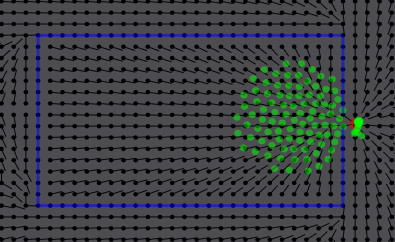
\includegraphics{UG} %treba malo obraditi slike i dati im nazive i labele
\
\end{figure}

Najprimetniji fenomen koji se javlja u paničnim situacijama je stvaranje uskih grla, odnosno gomilanje velikog broja ljudi na izlazima. Ovo je očeivano jer je osnovni cilj ljudi prilikom evakuacije da se sklone od opasnosti, dnosno napuste prostoriju.

\item Stvaranje uskog grla na proširenjima

\begin{figure}
\centering
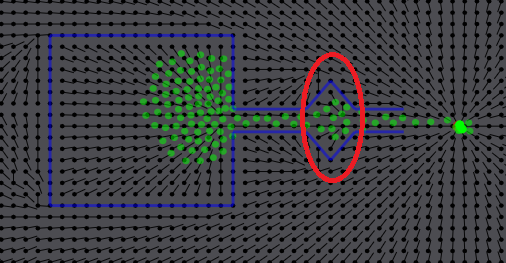
\includegraphics{Guzva}
\caption{Caption}
\label{fig:my_label}
\end{figure}

Ukoliko se u nekom hodniku nalazi proširenje, kao na slici refslike i preferirana brzina pešaka je dovoljno velika umesto očekivanog rasterećenja i ubrzavanja izlaska pešaka iz prostorije dolazi do stvaranja uskog grla. Ovaj fenomen se može objasniti time što na početku proširnja pešaci pokušavaju da prestignu jedni druge i tako se udaljavaju od glavnog toka. Kada na kraju proširenja pešaći ponovo pokušavaju da uđu u glavni tok dolazi do stvaranja uskog grla.

\item Evkuacija ljudi u malim grupama

\begin{figure}
\centering
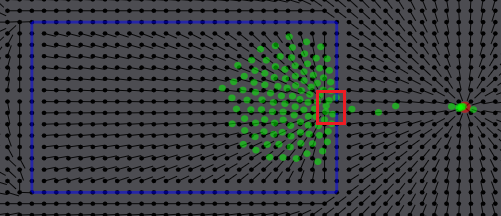
\includegraphics{SCGrupa1}
\caption{Caption}
\label{fig:my_label2}
\end{figure}


Pri visokim preferiranim brzinama pešaka, njihov izlazak iz prostorije postaje neravnomeran, odnosno pešaci napuštaju prostoriju u izdvojenim malim grupama. Takođe, tada se na izlazu iz prostorije javlja začepljenje u obliku luka (takvo začepljenje je obeleženo na slici ref). Do formiranja začepljenja u obliku luka na izlazu dolazi usled međusobnog guranja pešaka i sile kojom deluju jedni na druge pri fizičkom kontaktu. Do izlaska male grupe pešaka iz prostorije dolazi pri "rušenju" luka na izlazu. Primećeno je na stvaranje lučnih začepljenja znatno veći uticaj ima širina izlaza nego preferirana brzina pešaka.

\item Zanemarivanje slobodnih izlaza

%treba napraviti sliku za ovo
Kada je znanje pešaka o okolini u kojoj se nalaze malo (npr. kada je prostorija koju treba da napuste puna dima) uočeno je da se pešaci gomilaju na jednom izlazu, često zanemarivajući druge, slobodne izlae kroz koje bi napustili prostoriju za kraće vreme. Ovaj fenomen je u skladu sa zakljukom empirijskih istraživanja da su ljudima privlačnije one rute koji koristi veći broj drugih ljudi. Treba napomenuti da ni isključivo individualističko ponašanje u situacijama kada je znanje o okolini malo prema našem modelu ne daje rezultate jer pešak tada izlaz može naći samo slučajno, već je najefikasniji oblik ponašanja kombinacija individualističkog i kolektivnog ponašanja.

%\item Formiranje traka pri prolasku kroz hodnik

\end{enumerate}
    
    \label{fenomeni}

\section{Genetski algoritam}\label{GA}

Ranije smo spomenuli da se vreme evakuacije smanjuje ukoliko se na izlaz iz prostorije postavi nekakva prepreka, koja će da razbije i podeli bujicu pešaka. Ipak, nigde u literaturi nije specificirano koji je zapravo optimalan oblik te prepreke, već je korišćen oblik koji po autorovoj intuiciji daje najbolje rezultate. Ali, s obzirom na to da je sama ideja postavljanja prepreke donekle kontraintuitivna, glavni doprinos ovog rada je algoritamsko određivanje tog oblika.

S obzirom na to da ne možemo da ispitamo svaki mogući oblik (ima ih beskonačno mnogo), moramo se zadovoljiti približnim rešavanjem datog problema. Genetski algoritmi su jedna od klasa algoritama pogodnih baš za tu svrhu - optimizaciju neke \emph{fitness funkcije} (vremena izlaska) na nekom domenu, tzv \emph{prostoru pretraživanja} (u našem slučaju, skupu svih mogućih poligona u ravni).

Tok algoritma je sledeći:
\begin{enumerate}
\item Na slučajan način se generiše početni skup rešenja (\emph{jedinki}, na terminologiji genetskih algoritama) - poligona u ravni
\item Za svaku jedinku se pokrene simulacija sa tim poligonom kao preprekom na izlazu. Fitness te jedinke je recipročna vrednost ukupnog simuliranog vremena potrebnog za evakuaciju svih pešaka.
\item Sve jedinke (\emph{populacija}) se sortiraju prema fitness-u i "loše" jedinke sa malim fitness-om (prevelikim ukupnim vremenom izlask) se izbacuji iz populacije. Ovaj korak se u literaturi naziva \emph{selekcija}.
\item Jedinke koje su opstale, učestvuju u procesu \emph{ukrštanja}: iz populacije se biraju parovi jedinki koje će se ukrstiti i dati novu jedinku - \emph{potomak}, nastalu kombinovanjem poligona svoja dva \emph{roditelja}. Verovatnoća da neka jedinka bude odabrana je srazmerna njenom fitness-u.
\item Konačno, jedan deo jedinki u populaciji se dobija \emph{mutacijom} slučajno odabrane jedinke iz prethodne \emph{generacije}. Tako se u populaciju unosi mala količina raznovrsnosti, koja pomaže algoritmu da se ne zaustavi u nekom lokalnom optimumu.
\item Koraci 2 - 5 se ponavljaju dok populacija ne konvergira ili se izračuna određeni unapred zadati broj generacija
\end{enumerate}

Ovaj postupak je u velikoj meri tačan i za sve ostale genetske algoritme, i ostavlja mnogo prostora za slobodnu interpretaciju. Zato ćemo u sledećem delu dati konkretnu reprezentaciju jedne jedinke, kao i opise korišćenih genetskih operatora (selekcije, ukrštanja i mutacije). U radu su korišćena dva različita načina za predstavljanje prepreka: polarni $n$-tougao i kvadratna rešetka.

\subsection{Genetski operatori - $n$-tougao}

Svaka jedinka - mnogougao ima fiksiran broj ivica, $n$, i parametrizovan je sa $n$ realnih brojeva, $(r_0, r_1, \dots, r_{n-1})$. Temena tog mnogougla su tačke
$$\left(r_i \cos\left(\frac{2\pi i}{n}\right), r_i \sin\left(\frac{2\pi i}{n}\right)\right), \qquad i=0,\dots,n-1,$$
translirane na odgovarajuće mesto, ispred izlaza iz prostorije. Sa jedne strane, uz dovoljno veliko $n$ se na ovaj način može aproksimirati većina nama "interesantnih" poligona, a sa druge, na ovakvoj reprezentaciji se mogu koristiti mnogi "klasični" genetski operatori iz literature, koji pretpostavljaju međusobnu nezavisnost pojedinačnih komponenti vektora koji predstavlja jednu jedinku.

\begin{description}
\item[Selekcija] je primitivna, i prosto izbacuje sve jedinke sa fitness-om koji je više od 5 puta manji od najbolje jedinke. Konstanta 5 je odabrana proizvoljno i služi za odbacivanje onih prepreka koje u potpunosti blokiraju izlaz, i čije odgovarajuće jedinke imaju fitness 0.
\item[Ukrštanje] dve jedinke 
$$r^a = (r^a_0, r^a_1, \dots, r^a_{n-1}) \text{ i } r^b=(r^b_0, r^b_1, \dots, r^b_{n-1})$$ je sekvencijalno: Bira se proizvoljna početna pozicija $p$, $0\leq p < n$ i dužina $l$, $0 < l < n $. Nova jedinka $r = (r_0, r_1, \dots, r_{n-1})$ je definisana na sledeći način:
$$
r_i = 
\begin{cases}
    r^a_i & \text{za } i=p, p+1, \dots, p+l-1\\
    r^b_i & \text{inače}
\end{cases}.
$$
Pri tome je $r^a_i = r^a_{i-n}$, za $i\geq n$.
\item[Mutacija] sa malom verovatnoćom na proizvoljan način bira jednu od komponenata vektora jedinke i množi je sa slučajnom promenljivom $x$, koja ima Gausovu raspodelu sa centrom u 1.
\end{description}

\subsection{Genetski operatori - rešetka}

Za slučaj da se optimalno rešenje ne može predstaviti u gorenavedenom obliku, implementirali smo i alternativno predstavljanje prepreke, kao kvadratne rešetke $n\times n$ fiksiranih dimenzija (u smislu dužine i širine u simuliranom svetu), koja ima neka prohodna i neka neprohodna polja. Jedinka je predstavljena kvadratnom matricom $(b_{ij})$, gde je
$$
b_{ij} = 
\begin{cases}
    0 & \text{ako je polje prohodno}\\
    1 & \text{ako nije}
\end{cases}
$$

Genetski operatori su sledeći:
\begin{description}
\item[Selekcija] je ista kao u prethodnom slučaju, jer je nezavisna od reprezentacije jedinke.
\item[Ukrštanje] jedinki $(b^a_{ij})$ i $(b^b_{ij})$:
$$
b_{ij} = 
\begin{cases}
    b^a_{ij} & \text{sa verovatnoćom } \frac{f_a}{f_a+f_b}\\
    b^b_{ij} & \text{sa verovatnoćom } \frac{f_b}{f_a+f_b}
\end{cases},
$$
pri čemu su $f_a$ i $f_b$ fitness funkcije prve i druge jedinke, redom. Primetimo da ako je $ b^a_{ij} = b^b_{ij}$, tada će biti i $b_{ij} = b^a_{ij} = b^b_{ij}$.
\item[Mutacija]: sa malom verovatnoćom, neko od neprohodnih polja na ivici prepreke postaje prohodno.
\end{description}

\section{Rezultati i diskusija}

Dobijeni rezultati se mogu podeliti u dve kategorije, kvalitativnu i kvantitativnu. Sa kvalitativne strane, replicirani su fenomeni uočeni u drugim modelima, kao što je zanemarivanje slobodnih izlaza i stvaranje uskog grla na proširenjima. Više o svim reprodukovanim fenomenima je bilo reči u odeljku \ref{fenomeni}, i na tome se više nećemo zadržavati.

Sa kvalitativne strane, rezultati se ponovo dele na dve grupe: oni dobijeni iz pojedinačne simulacije pokrenute za neke parametre interesantne po mišljenju autora, kao i oni dobijeni pokretanjem genetskog algoritam za optimizaciju pešačkih zona.

Iz  prve grupe su reprezentativni grafici zavisnosti evakuisanih pešaka od vremena, sa kojih se mogu uočiti fenomeni poput napuštanja prostorije u mailm grupama. Takođe pokretanjem pojedinačne simulacije je potvrđena i hipoteza da prisustvo prepreke na izlazu smanjuje vreme izlaska iz prostorije.

% slika grafika zavisnosti broja pesaka od vremena
% slike terena sa preprekom i njegovo vreme izlaska, i teren bez prepreke i njegovo vreme

Daleko su interesantniji rezutati dobijeni genetskim algoritmom, iz kojih smo videli da genetski algoritam konvergira, i da može da se primeni na dati problem. Predstavljamo rezultate genetskog algoritma za obe reprezentacije jedinki. Ukoliko drugačije nije naglašeno, genetski algoritam se izvršavao kroz 50 generacija, sa 20 jedinki.

%slika početnog terena sa regijom gde se spawnuju pesaci

\subsection*{Polarni mnogouglovi}

% grafik konvergencije najboljeg resenja za razlicite seedove
% slika optimalnog (ih?) resenja

\subsection*{Kvadratna rešetka} 

% grafik konvergencije najboljeg i najgoreg rezultata
% slika optimalnog resenja

Iako razlike u oba slučaja nisu prevelike, u kritičnim situacijama (požar, ...) su i najmanja ubrzanja procesa evakuacije uvek dobrodošla, pa je stoga opravdano postavljati ovakvu prepreku na izlazu iz neke prostorije.

Autori nemaju objašnjenje zašto rešenja dobijena algoritmom izgledaju baš tako, ali je moguće da oni ukazuju na neophodnost postavljanja dve prepreke-stuba za dostizanje još boljih rezultata. Nažalost, zbog ograničenog vremena ta hipoteza nije proverena.

Još jedna mogućnost jeste implementacija dvoslojnog genetskog algoritma, u kojoj se rezultati iz različitih pokretanja genetskog algoritma koriste kao početna populacija za još jedno izvršavanje algoritma. Na taj način je moguće da će doći do ukrštanja lokalnih optimuma, i eventualnog pronalaska globalnog.

\section{Zaključak}

U radu je prestavljen proširen model socijalnih sila, i genetski algoritam za optimizaciju pešačkih zona. Nakon proveravanja verodostojnosti simulacije ispitivanjem javljanja nekih uočenih sociološkoh fenomena, genetskim algoritmom je utvrđen optimalan izgled prepreke koju je potrebno postaviti na izlaz iz neke prostorije, da bi se minimizovalo vreme evakuacije svih pešaka.

\bibliographystyle{apalike}  
\begin{scriptsize}
\bibliography{bibliography}
\end{scriptsize}

\end{document}